%%%%%%%%%%%%%%%%%%%%%%%%%%% asme2ej.tex %%%%%%%%%%%%%%%%%%%%%%%%%%%%%%%
% Template for producing ASME-format journal articles using LaTeX    %
% Written by   Harry H. Cheng, Professor and Director                %
%              Integration Engineering Laboratory                    %
%              Department of Mechanical and Aeronautical Engineering %
%              University of California                              %
%              Davis, CA 95616                                       %
%              Tel: (530) 752-5020 (office)                          %
%                   (530) 752-1028 (lab)                             %
%              Fax: (530) 752-4158                                   %
%              Email: hhcheng@ucdavis.edu                            %
%              WWW:   http://iel.ucdavis.edu/people/cheng.html       %
%              May 7, 1994                                           %
% Modified: February 16, 2001 by Harry H. Cheng                      %
% Modified: January  01, 2003 by Geoffrey R. Shiflett                %
% Butchered: October 15, 2014 by John Karasinski                     %
% Use at your own risk, send complaints to /dev/null                 %
%%%%%%%%%%%%%%%%%%%%%%%%%%%%%%%%%%%%%%%%%%%%%%%%%%%%%%%%%%%%%%%%%%%%%%

%%% use twocolumn and 10pt options with the asme2ej format
\documentclass[twocolumn,10pt]{asme2ej}

\usepackage{epsfig} %% for loading postscript figures
\usepackage{amsmath}
\usepackage{graphicx}
\usepackage{grffile}
\usepackage{pdfpages}
\usepackage{algpseudocode}

% Default fixed font does not support bold face
\DeclareFixedFont{\ttb}{T1}{txtt}{bx}{n}{12} % for bold
\DeclareFixedFont{\ttm}{T1}{txtt}{m}{n}{12}  % for normal

% Custom colors
\usepackage{color}
\usepackage{listings}
\usepackage{framed}
\usepackage{caption}
\captionsetup[lstlisting]{font={small,tt}}

\definecolor{mygreen}{rgb}{0,0.6,0}
\definecolor{mygray}{rgb}{0.5,0.5,0.5}
\definecolor{mymauve}{rgb}{0.58,0,0.82}

\lstset{ %
  backgroundcolor=\color{white},   % choose the background color; you must add \usepackage{color} or \usepackage{xcolor}
  basicstyle=\ttfamily\footnotesize, % the size of the fonts that are used for the code
  breakatwhitespace=false,         % sets if automatic breaks should only happen at whitespace
  % breaklines=true,                 % sets automatic line breaking
  captionpos=b,                    % sets the caption-position to bottom
  commentstyle=\color{mygreen},    % comment style
  deletekeywords={...},            % if you want to delete keywords from the given language
  escapeinside={\%*}{*)},          % if you want to add LaTeX within your code
  extendedchars=true,              % lets you use non-ASCII characters; for 8-bits encodings only, does not work with UTF-8
  frame=single,                    % adds a frame around the code
  keepspaces=true,                 % keeps spaces in text, useful for keeping indentation of code (possibly needs columns=flexible)
  columns=flexible,
  keywordstyle=\color{blue},       % keyword style
  language=Python,                 % the language of the code
  morekeywords={*,...},            % if you want to add more keywords to the set
  numbers=left,                    % where to put the line-numbers; possible values are (none, left, right)
  numbersep=5pt,                   % how far the line-numbers are from the code
  numberstyle=\tiny\color{mygray}, % the style that is used for the line-numbers
  rulecolor=\color{black},         % if not set, the frame-color may be changed on line-breaks within not-black text (e.g. comments (green here))
  showspaces=false,                % show spaces everywhere adding particular underscores; it overrides 'showstringspaces'
  showstringspaces=false,          % underline spaces within strings only
  showtabs=false,                  % show tabs within strings adding particular underscores
  stepnumber=1,                    % the step between two line-numbers. If it's 1, each line will be numbered
  stringstyle=\color{mymauve},     % string literal style
  tabsize=4,                       % sets default tabsize to 2 spaces
}

\title{Case Study \# 5: Two-Species Diffusion-Diurnal Kinetics}

\author{John Karasinski
    \affiliation{
  Graduate Student Researcher\\
  Center for Human/Robotics/Vehicle Integration and Performance\\
  Department of Mechanical and Aerospace Engineering\\
  University of California\\
  Davis, California 95616\\
    Email: karasinski@ucdavis.edu
    }
}

\begin{document}
\maketitle

%%%%%%%%%%%%%%%%%%%%%%%%%%%%%%%%%%%%%%%%%%%%%%%%%%%%%%%%%%%%%%%%%%%%%%
\section{Problem Description}

%%%%%%%%%%%%%%%%%%%%%%%%%%%%%%%%%%%%%%%%%%%%%%%%%%%%%%%%%%%%%%%%%%%%%%
\section{Numerical Solution Approach}

%%%%%%%%%%%%%%%%%%%%%%%%%%%%%%%%%%%%%%%%%%%%%%%%%%%%%%%%%%%%%%%%%%%%%%
\section{Results Discussion}


\begin{table}[tbh]
\begin{center}
\begin{tabular}{| l | r |}
\hline
Solver & Time (s) \\
\hline
dop853 & 11092 \\
dopri5 & 10069 \\
bdf    & 13237 \\
\hline
\end{tabular}
\caption{10 days solution}
\label{10_days}
\end{center}
\end{table}

\begin{table}[tbh]
\begin{center}
\begin{tabular}{| l | r |}
\hline
Solver & Time (s) \\
\hline
dop853 & 1120 \\
dopri5 & 1025 \\
bdf    & 1318 \\
\hline
\end{tabular}
\caption{24 hours solution}
\label{24_hours}
\end{center}
\end{table}

\begin{figure}[thb]
\begin{center}
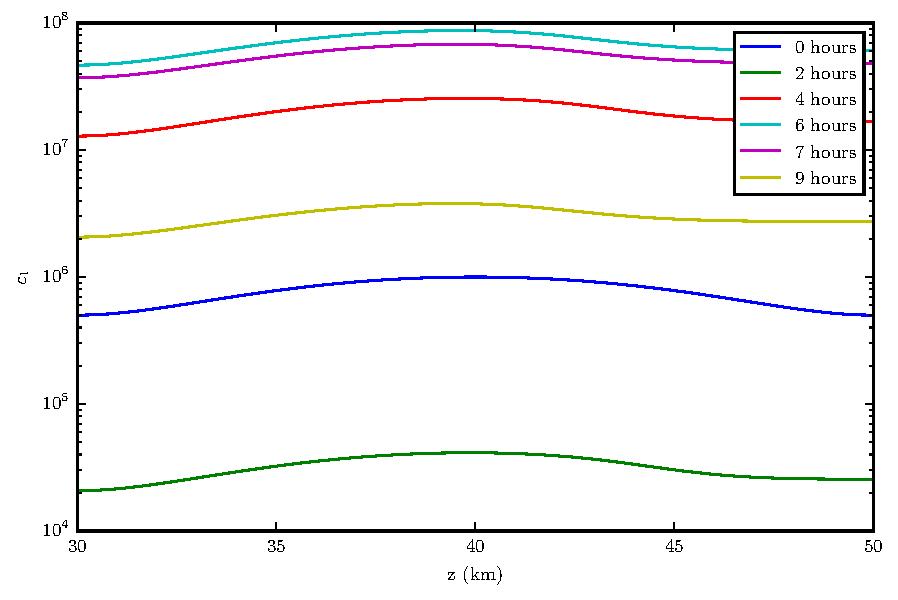
\includegraphics[width=0.5\textwidth]{figure/bdf c1.pdf}
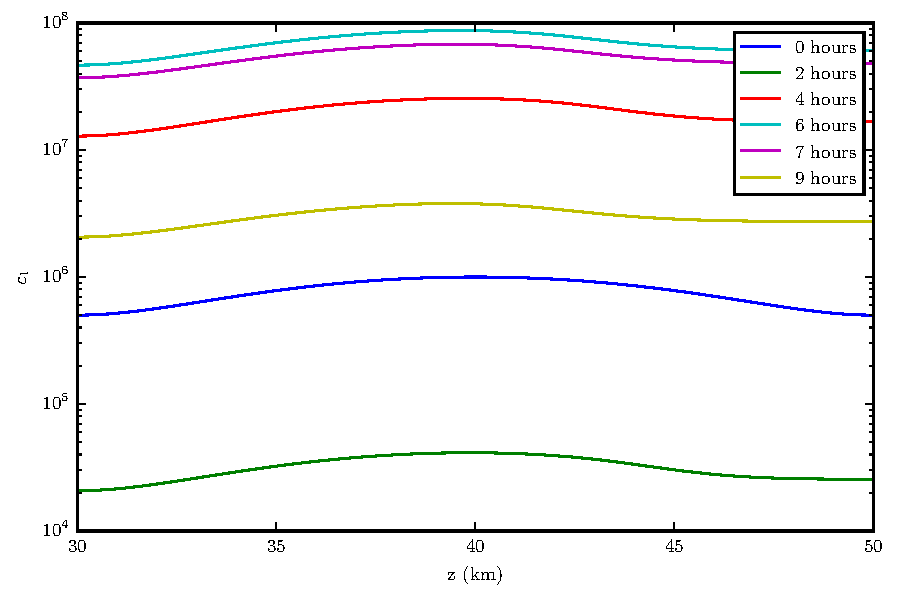
\includegraphics[width=0.5\textwidth]{figure/dop853 c1.pdf}
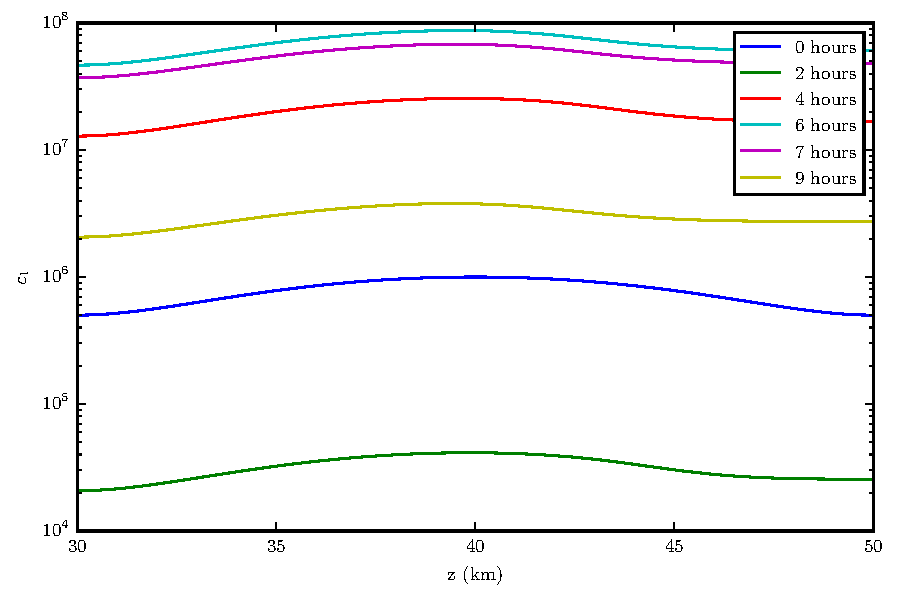
\includegraphics[width=0.5\textwidth]{figure/dopri5 c1.pdf}
\caption{Results from bdf, dop853, and dopri5 solvers of $c_1$ vs. z at $t = $ 0, 2, 4, 6, 7, and 9 hours}
\label{c1}
\end{center}
\end{figure}

\begin{figure}[thb]
\begin{center}
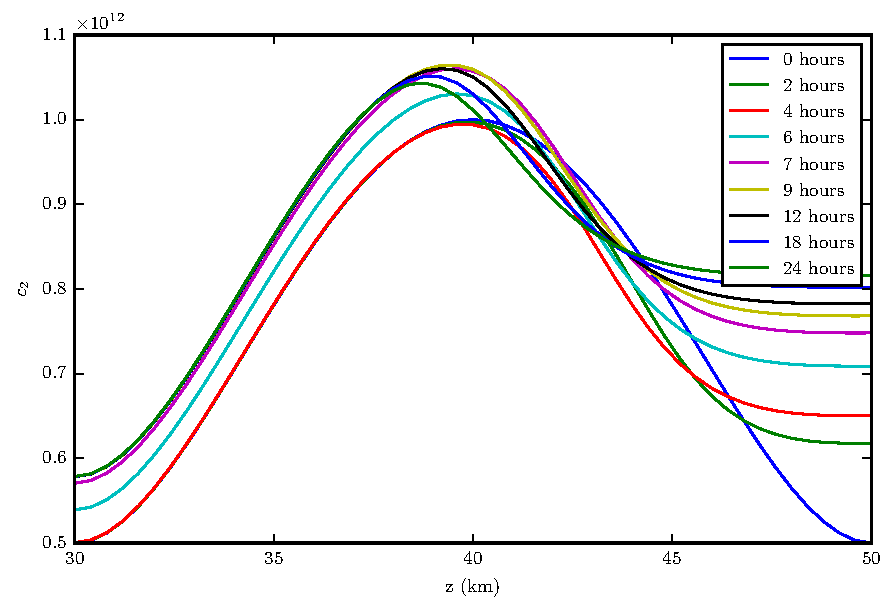
\includegraphics[width=0.5\textwidth]{figure/bdf c2.pdf}
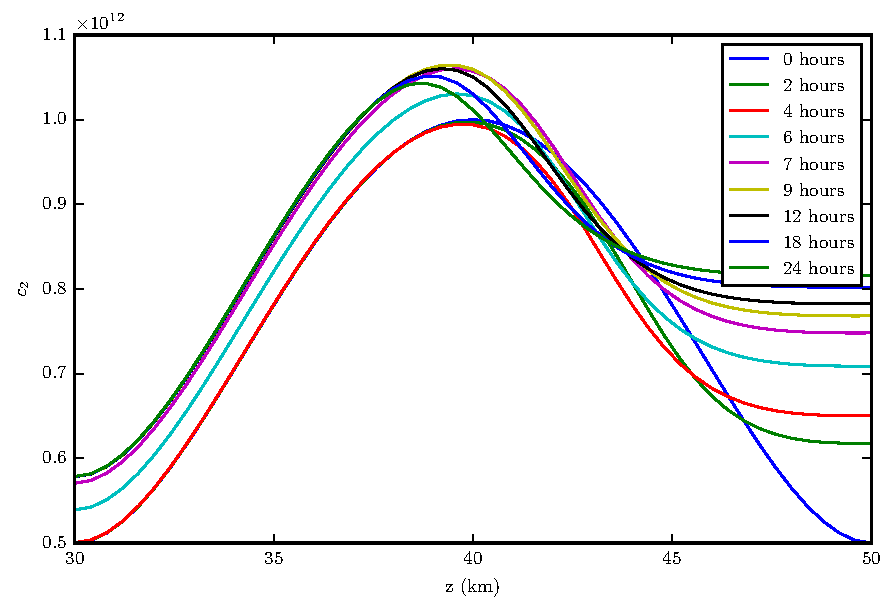
\includegraphics[width=0.5\textwidth]{figure/dop853 c2.pdf}
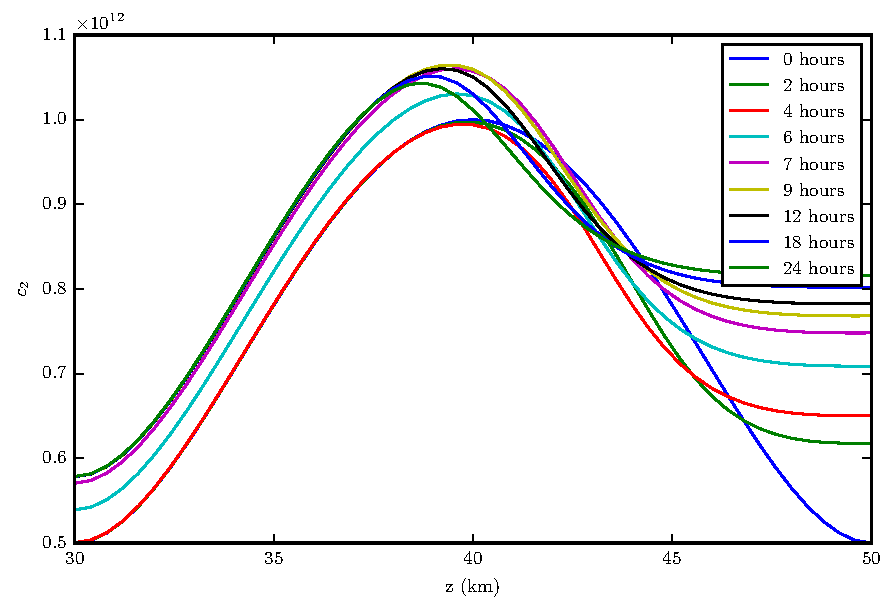
\includegraphics[width=0.5\textwidth]{figure/dopri5 c2.pdf}
\caption{Results from bdf, dop853, and dopri5 solvers of $c_2$ vs. z at $t = $ 0, 2, 4, 6, 7, 9, 12, 18, and 24 hours}
\label{c2}
\end{center}
\end{figure}

\begin{figure}[thb]
\begin{center}
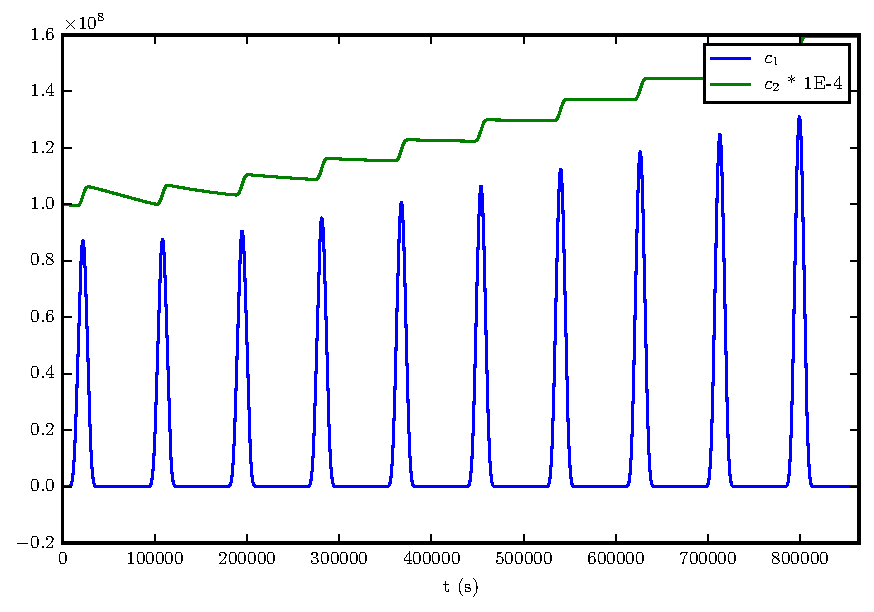
\includegraphics[width=0.5\textwidth]{figure/bdf time.pdf}
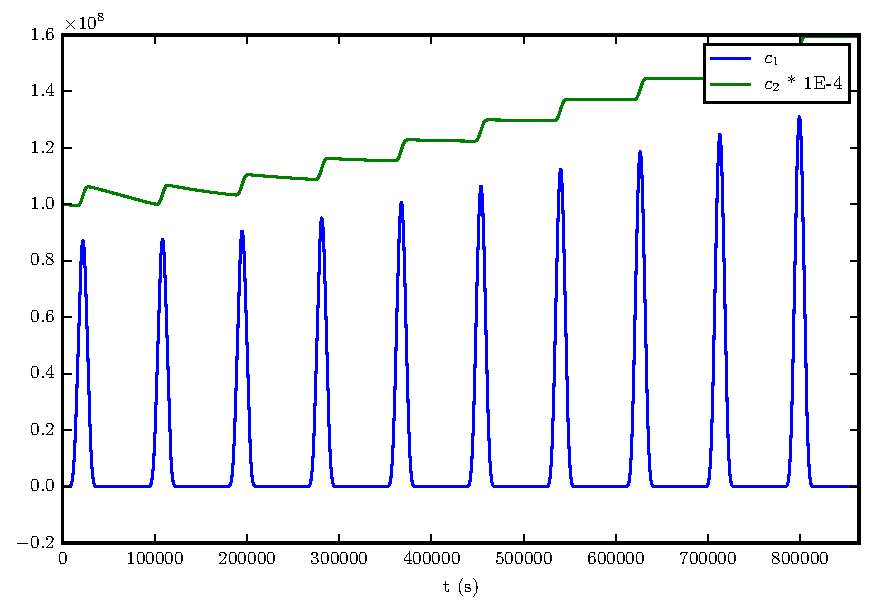
\includegraphics[width=0.5\textwidth]{figure/dop853 time.pdf}
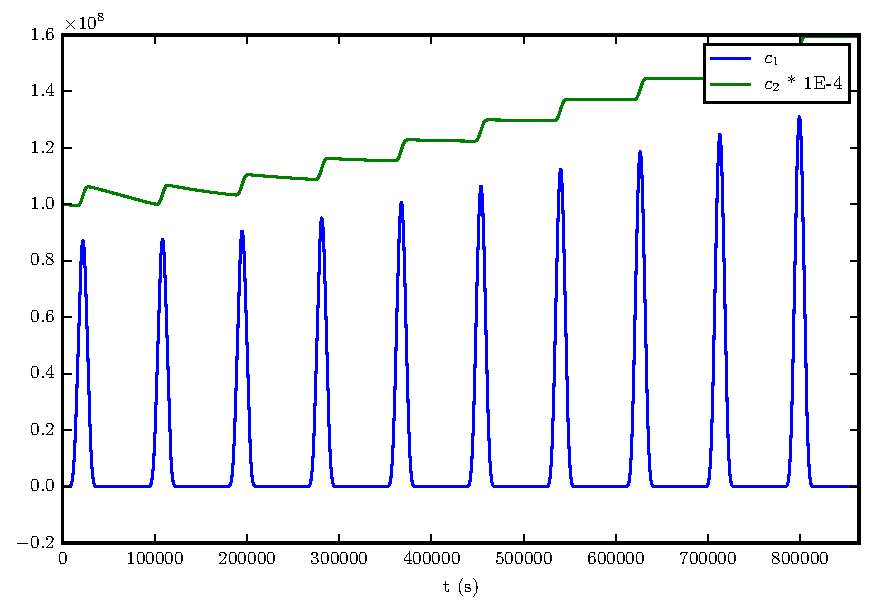
\includegraphics[width=0.5\textwidth]{figure/dopri5 time.pdf}
\caption{Results from bdf, dop853, and dopri5 solvers of $c_1$ and $c_2$ vs. time (from 0 to 10 days) at $z = 40$ km}
\label{10 days}
\end{center}
\end{figure}

%%%%%%%%%%%%%%%%%%%%%%%%%%%%%%%%%%%%%%%%%%%%%%%%%%%%%%%%%%%%%%%%%%%%%%
\section{Conclusion}

%%%%%%%%%%%%%%%%%%%%%%%%%%%%%%%%%%%%%%%%%%%%%%%%%%%%%%%%%%%%%%%%%%%%%%
\nocite{*}
\bibliographystyle{asmems4}
\bibliography{asme2e}

%%%%%%%%%%%%%%%%%%%%%%%%%%%%%%%%%%%%%%%%%%%%%%%%%%%%%%%%%%%%%%%%%%%%%%
\clearpage
\onecolumn
\appendix       %%% starting appendix
\section*{Appendix A: Python Code}

\lstinputlisting[caption=Code to create solutions, language=Python]{../code/CaseStudy5.py}
\lstinputlisting[caption=Code to generate pretty plots, language=Python]{../code/PrettyPlots.py}

%%%%%%%%%%%%%%%%%%%%%%%%%%%%%%%%%%%%%%%%%%%%%%%%%%%%%%%%%%%%%%%%%%%%%%
\end{document}
